\documentclass[tikz, border=10pt]{standalone}
\usepackage[T1]{fontenc}
\usepackage[utf8]{inputenc}
\usepackage{lmodern}
\usepackage[table]{xcolor}
\definecolor{IntelBlue}{HTML}{0068B5}
\definecolor{IntelLightBlue}{HTML}{DDEEF9}
\definecolor{FpgaOrange}{HTML}{E67E22}
\definecolor{FpgaLight}{HTML}{FDEBD0}
\definecolor{HpsGreen}{HTML}{1A7A4A}
\definecolor{HpsLight}{HTML}{D5F5E3}
\definecolor{GrayBg}{HTML}{F2F3F4}
\definecolor{GrayBorder}{HTML}{AAB7B8}
\definecolor{PassGreen}{HTML}{D5F5E3}
\definecolor{PassGreenDark}{HTML}{1E8449}
\definecolor{RowAlt}{HTML}{F7F9FB}
\definecolor{SummaryBg}{HTML}{EBF5FB}
\definecolor{NodeFill}{HTML}{D6EAF8}
\definecolor{NodeBorder}{HTML}{1B4F72}
\definecolor{InitFill}{HTML}{E5E7E9}
\definecolor{InitBorder}{HTML}{717D7E}
\definecolor{SleepFill}{HTML}{FEF5E7}
\definecolor{SleepBorder}{HTML}{935116}
\definecolor{MsgFill}{HTML}{D1F2EB}
\definecolor{MsgBorder}{HTML}{0E6655}
\definecolor{TimeoutRed}{HTML}{C0392B}
\definecolor{BtnBlue}{HTML}{1A5276}
\definecolor{ArrowGray}{HTML}{717D7E}
\usepackage{tikz}
\usetikzlibrary{shapes.geometric, arrows.meta, positioning, fit, backgrounds, calc, decorations.pathreplacing, bending, shadows.blur}
\begin{document}
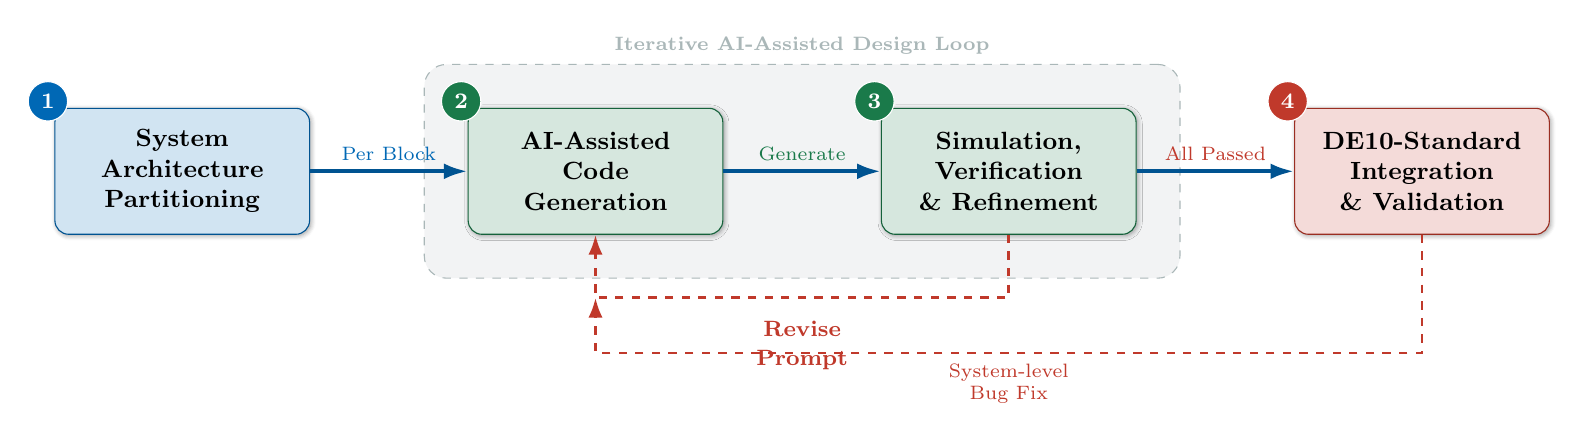
\begin{tikzpicture}[
  auto,
  node distance=2.2cm,
  mainblock/.style={
    rectangle,
    draw=#1!80!black,
    fill=#1!18,
    text width=3.0cm,
    align=center,
    rounded corners=5pt,
    minimum height=1.6cm,
    font=\small\bfseries,
    blur shadow={shadow blur steps=5,
                 shadow xshift=0.5pt,
                 shadow yshift=-0.5pt}},
  mainblock/.default=IntelBlue,
  fwd/.style={
    draw=IntelBlue!80!black,
    -{Latex[length=3mm,width=2mm]},
    line width=1.5pt},
  back/.style={
    draw=TimeoutRed,
    dashed,
    -{Latex[length=2.5mm,width=1.8mm]},
    line width=1.0pt},
  badge/.style={
    circle,
    draw=white,
    fill=#1,
    text=white,
    font=\footnotesize\bfseries,
    inner sep=1.5pt,
    minimum size=0.5cm},
  badge/.default=GrayBorder,
]

\node[mainblock=IntelBlue] (arch)
  {System\\Architecture\\Partitioning};

\node[mainblock=HpsGreen, right=2.0cm of arch] (aigen)
  {AI-Assisted\\Code\\Generation};

\node[mainblock=HpsGreen, right=2.0cm of aigen] (refine)
  {Simulation,\\Verification\\\& Refinement};

\node[mainblock=TimeoutRed, right=2.0cm of refine] (deploy)
  {DE10-Standard\\Integration\\\& Validation};

\node[badge=IntelBlue,
      above left=-0.1cm and -0.1cm of arch.north west]
  {\textbf{1}};
\node[badge=HpsGreen,
      above left=-0.1cm and -0.1cm of aigen.north west]
  {\textbf{2}};
\node[badge=HpsGreen,
      above left=-0.1cm and -0.1cm of refine.north west]
  {\textbf{3}};
\node[badge=TimeoutRed,
      above left=-0.1cm and -0.1cm of deploy.north west]
  {\textbf{4}};

\begin{scope}[on background layer]
  \node[fill=GrayBg,
        draw=GrayBorder,
        dashed,
        rounded corners=8pt,
        fit=(aigen)(refine),
        inner sep=0.55cm,
        label={[font=\scriptsize\bfseries\color{GrayBorder}]
               above:Iterative AI-Assisted Design Loop}]
    (loopbox) {};
\end{scope}

\draw[fwd] (arch)   --
  node[above, font=\scriptsize\color{IntelBlue}]  {Per Block}  (aigen);
\draw[fwd] (aigen)  --
  node[above, font=\scriptsize\color{HpsGreen}]   {Generate}   (refine);
\draw[fwd] (refine) --
  node[above, font=\scriptsize\color{TimeoutRed}] {All Passed} (deploy);

\draw[back]
  (refine.south) -- ++(0,-0.8)
  -- node[below=7pt, font=\footnotesize\bfseries\color{TimeoutRed}, align=center,
          fill=white, inner sep=1pt]
       {Revise\\[1pt]Prompt}
  ($(aigen.south)+(0,-0.8)$) -- (aigen.south);

\draw[back]
  (deploy.south) -- ++(0,-1.5)
  -- node[below, font=\scriptsize\color{TimeoutRed}, align=center]
       {System-level\\Bug Fix}
  ($(aigen.south)+(0,-1.5)$) -- ++(0,0.7);

\end{tikzpicture}
\end{document}
